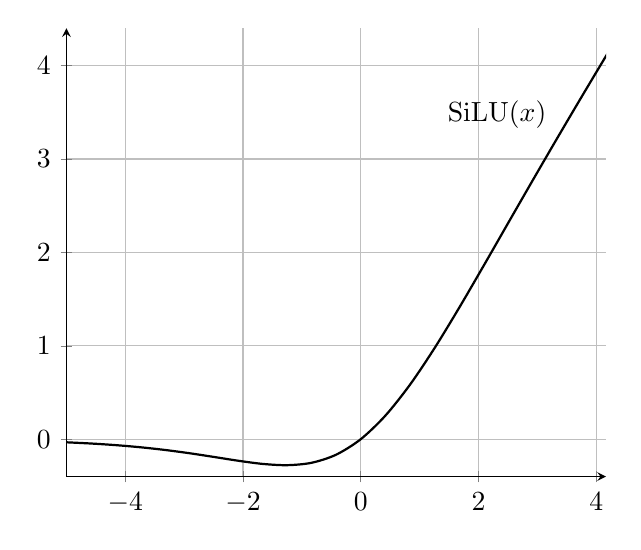
\begin{tikzpicture}
    \begin{axis}[
        % xlabel = $x$,
        % ylabel = $ReLU\left(x\right)$,
        ymin = -0.4,ymax = 4.4,
        domain = -6:6,
        grid=both,
        % width=5.5cm,
        smooth,
        axis lines = left,
    ]
  
    \addplot[color=black,domain=-5:5,thick]{x/(1+exp(-x))} node[pos=0.8,anchor=south east]{SiLU$(x)$};
    %   \addplot[color=blue]{tanh(x)};
    %   \addplot[color=blue,dashed,domain=-1:1,thin]{x};
    \end{axis}
    % \draw (0,-1) node [inner sep=0.75pt]{
    %   $\sigmoid{x} =\frac{1}{1+e^{-x}}$
    % };
\end{tikzpicture}
